\documentclass[12pt]{article}
\usepackage[utf8]{inputenc}
\usepackage[brazil]{babel}
\usepackage{graphicx}
\usepackage{cancel}
\usepackage{mathtools}
\usepackage{float}
\usepackage{epsfig}
\usepackage{xcolor}
\usepackage{multicol}
\usepackage[sorting=none]{biblatex}
\addbibresource{src/references/references.bib}
\usepackage{mathptmx} %para Times Roman
\usepackage{amsmath,amssymb}
\usepackage{setspace} \setstretch{1.5} %para espaçamento 1.15
\usepackage{geometry} %para definir a geometria da página
\usepackage{booktabs} %pacote para tabelas
\usepackage{caption} %Legendas das figuras
\geometry{left=2cm,right=2cm, top=2cm, bottom=2cm} %margens da página
\setlength{\parindent}{1cm} %tamanho do parágrafo
\usepackage{indentfirst} %primeiro parágrafo do \section
\usepackage{fancyhdr}
\usepackage{url}
\usepackage{listings}
\pagestyle{fancy}
\fancyhf{}
\lhead{Entrega Final - Reinforcement Learning}
\rfoot{\thepage}


\everymath{\displaystyle}
\newtheorem{exem}{Exemplo}

\begin{document}

\begin{titlepage}
    \vfill
	\begin{center}
    
\includegraphics[scale=1.0]{src/img/insper-cover.png}\\
	\textbf{AGENTES AUTÔNOMOS E REINFORCEMENT LEARNING \\ [0.05cm]ELETIVA}

	\vspace{0.6cm}
	\vspace{4cm}
	{\huge \textbf{Projeto Final - Entrega Final}}\vspace{8mm}
	
	{\large \textbf{Caio Emmanuel}}\\[2.5cm]
	
		\hspace{.45\textwidth} %posiciona a minipage
	   \begin{minipage}{.5\textwidth}
	   Entrega final contendo implementação e resultados finais sobre um agente autônomo desenvolvido para o jogo Doom.\\[0.1cm]
	  \end{minipage}
	  \vfill
	
	\textbf{São Paulo}
	
	\textbf{Junho de 2022}
	\end{center}
	
\end{titlepage}
\pagebreak
\tableofcontents
\pagebreak

\section{Introdução}

\subsection{Contexto}

Este trabalho foi realizado sobre o ambiente da biblioteca \textit{Python} chamada \textit{ViZDoom}\cite{vizdoom}, uma biblioteca criada para integrar os cenários recriados de \textit{ZDoom}\cite{zdoom} com a estrutura de \textit{environments} da biblioteca \textit{gym}\cite{gym}.

Os agentes criados foram treinados sobre os cenários da categoria \textit{basics}, ou seja, eles possuem apenas uma sala pequena, com um ou alguns poucos monstros e a movimentação é limitada a um único grau de liberdade (esquerda-direita).

\subsection{Objetivo}

O objetivo desse trabalho é implementar e analisar a performance de um agente autônomo atuando sobre os cenários \textit{basics} da biblioteca \textit{ViZDoom}.

\section{Implementação}

O código principal para implementar o agente está no arquivo \textit{agent.py} no repositório que foi enviado junto desse arquivo. Os parâmetros importantes que forem citados estarão configurados no arquivo \textit{constants.py} e algumas funções que forem citadas estarão no arquivo \textit{utils.py}.

\subsection{Agente}

O agente desenvolvido utiliza o algoritmo \textit{Double Deep Q-Learning}\cite{vanhasselt2015deep} que consiste de utilizarmos duas redes neurais para simular os valores produzidos por uma \textit{Q-Table} no algoritmo clássico \textit{Q-Learning}. Onde uma das redes gera os valores da \textit{Q-Table} mas seus pesos são atualizados com menos frequência que a outra rede, que é atualizada a cada iteração do treinamento, mas produz valores com uma maior variação por conta disso.

Para isso foi utilizado o módulo \textit{PyTorch}.

\subsubsection{Rede neural}

A topologia da rede neural utilizada foi uma topologia convolucional, aqui não houve tanta preocupação em construir essa topologia visto que o foco era a performance do algoritmo de treinamento do agente e não da rede neural e, portanto, foi utilizada a topologia padrão dos exemplos da documentação do \textit{Pytorch} sobre \textit{Convolutional Networks} adaptada para os frames do jogo.

A rede neural consiste de quatro camadas de convolução e duas \textit{fully-connected} ao fim.

\subsubsection{Hiperparâmetros}

Sobre os hiperparâmetros, eles podem ser vistos em `constants.py` como dito, mas não há nada de especial sobre eles e foram escolhidos os mesmos que o tutorial do \textit{ViZDoom}.

O único hiperparâmetro que é importante comentar é o número de \textit{epochs} de treinamento. Segundo os próprios desenvolvedores, e conforme verificado durante o treinamento, um número muito alto de \textit{epochs}, superior a 20 (vinte), reduz a capacidade de aprendizado do agente e este até mesmo começa a regredir. Para 20 \textit{epochs} o \textit{score} do agente converge para algo entre 70 e 80.

\subsection{Pré-processamento}

Os \textit{frames} do jogo são preprocessados para diminuir a dimensão do \textit{input} da rede neural, necessitando de menos pesos para serem atualizados e, consequentemente, acelerando o treinamento. O pré-processamento é simples e constitui basicamente de diminuir as dimensões da imagem para outra dimensão especificada e retirar as três dimensões de cores, visto que as cores não traduzem nenhuma informação relevante.

\subsection{Treinamento}

O treinamento é semelhante ao proposto pelo \textit{paper} original sobre \textit{Double Deep Q-Learning}, ou seja, são gerados um número de \textit{batch frames}, em seguida os pesos da rede principal são treinados tendo como entrada esses \textit{frames} e os respectivos valores da \textit{Q-Table} produzidos pela rede \textit{target} que só será atualizada após algumas épocas com os pesos da rede principal.

Nesse caso em especial, foi adicionado um teste após cada treinamento, para verificar-se com novos \textit{frames} o desempenho do agente.

Os valores dos \textit{scores} são salvos para então produzir um gráfico com a evolução destes entre as \textit{epochs}.

\section{Resultados}

Os resultados podem ser verificados de duas formas.

Ao fim do treinamento, o agente irá jogar um número de jogos determinado em `constants.py` para verificar visualmente o comportamento deste.

Ainda, será gerado uma imagem com a evolução dos scores no tempo como a Figura 1.

\begin{figure}[H]
    \centering
    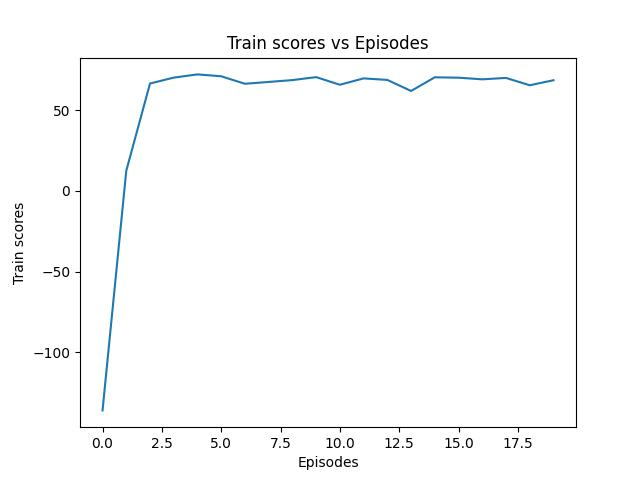
\includegraphics[scale=.8]{src/img/results-20-epochs.jpg}
    \caption{Average Score per Steps - Doom Agent}
\end{figure}

Em geral, o resultado foi satisfatório e cumpriu ao \textit{score} esperado segundo os comentários dos desenvolvedores que diziam que o \textit{score} deveria fixar entre 70 e 80 no caso ideal.

\pagebreak
\printbibliography
\pagebreak

\end{document}
